% !tex-engine = luatex
\documentclass[11pt]{lukereport}

% run with LuaLaTeX

%%%
% Next packages are for the template examples and can be removed.
\usepackage{lipsum}
%%%

%% dev, to be moved to class-file
\usepackage[singlelinecheck=false, labelsep=period, labelfont=bf]{caption}
\usepackage{tocloft} % adds toc dots
\renewcommand\cftchapaftersnum{.}% adds dot after chapter title in ToC
\renewcommand\cftchapdotsep{\cftdotsep}% adds leader dots from chapter titles to page numbers

% row space
%\linespread{1.1}

% Title Page
\title{Report title to be written here}
%\subtitle{Report specifier (if any)}
\author{Firstname Lastname}


\begin{document}
\maketitle

\begin{abstract}
\lipsum[2-3]
\end{abstract}

% if needed:
\setcounter{page}{5}

%\newpage
\setcounter{tocdepth}{2}



\tableofcontents

%\newpage


\chapter{Heading 1}

\lipsum[1]

\section{Heading 2 (TOC included)}

\lipsum[2]

\subsection{Heading 3 (TOC included)}
\begin{figure}[!hb]
	\centering
	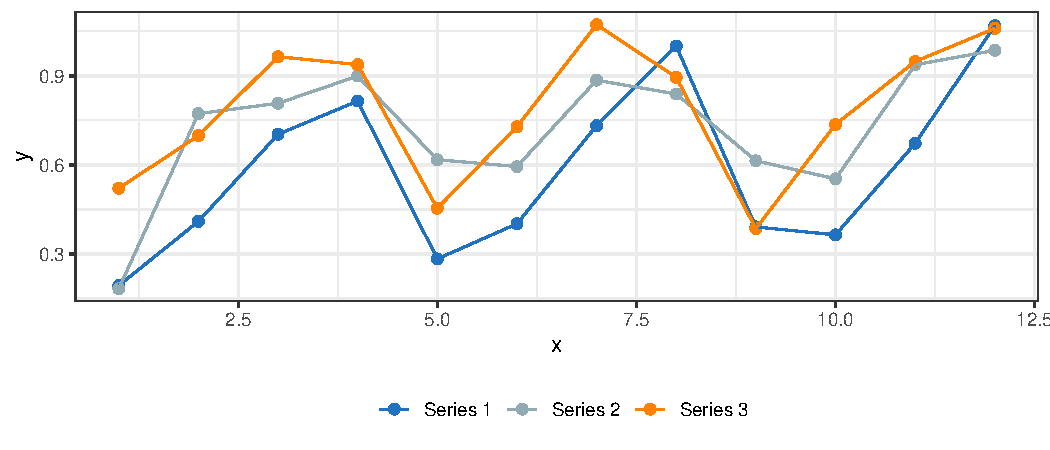
\includegraphics[width=.8\linewidth]{fig_ex1}
	\caption[short figure caption]{Long figure caption.}
	\label{fig:figex1}
\end{figure}

\lipsum[4]

\subsubsection{Heading 4 (TOC not included)}


\lipsum[6] See Figure \ref{fig:figex1}.


\chapter{Heading 1}

\lipsum[1]

\section{Heading 2 (TOC included)}

\lipsum[2]

\subsection{Heading 3 (TOC included)}
\lipsum[4-6]

\subsubsection{Heading 4 (TOC not included)}
\lipsum[5-6] See table \ref{tab:basic}.


 \begin{table}
 	\caption{Example of a basic table.}
 	\label{tab:basic}
% 	\centering
 	\fontfamily{phv}\fontseries{mc}\selectfont
 	
	\def\arraystretch{1.5} % bit more space
	\rowcolors{2}{black!5!white}{white}  % alternating colors
          \begin{tabular}{|=l|+c|+c|+c|+c|} % hack to get only first row text white
 		\hline
 		\rowcolor{lukedarkgray}\rowstyle{\color{white}\bf}
		& Column 1 & Column 2 & Column 3 & Column 4 \\
 		\hline
 		Row 1 & 1 & 2 & 3 & 4\\
 		\hline
 		Row 2 & 1 & 2 & 3 & 4\\
 		\hline
 		Row 3 & 1 & 2 & 3 & 4\\
 		\hline
 		Row 4 & 1 & 2 & 3 & 4\\
 		\hline
 	\end{tabular} 	

\end{table}



\end{document}      
